\documentclass[12pt, a4paper, final, fleqn]{article}
\usepackage{graphics, graphicx}
\usepackage{amsmath}
\usepackage{microtype}
\usepackage[english]{babel}
%\usepackage[round,numbers,comma,sort&compress]{natbib} % references as numbers
\usepackage[square,numbers,comma]{natbib} % refereces as text
\usepackage{a4wide}
\usepackage[normalem]{ulem}
\usepackage[colorlinks,citecolor=blue,filecolor=black,linkcolor=black,urlcolor=black]{hyperref}
\usepackage{color}
\usepackage{array}
\usepackage{colortbl}
\usepackage{tabularx}
\usepackage{booktabs}
\usepackage{lineno}
\usepackage{caption}  % to put caption outside figure env -- used for text boxes
\usepackage{setspace}  % to use double spacing
\graphicspath{{graphics/}}
\newcommand{\comment}[1]{}
\definecolor{nero}{rgb}{0., 0., 0.}
\definecolor{bianco}{rgb}{1, 1, 1}
\definecolor{andrea}{rgb}{0., 1., 1.}
\definecolor{grigio}{rgb}{.4, .4, .4}

\newcommand{\discA}[1]{\textcolor{andrea}{\sout{#1}}}
\newcommand{\chngA}[1]{\textcolor{andrea}{\textsf{\textbf{#1}}}}


\begin{document}

\begin{center}

\vspace*{2cm}

%{ \Large {\bf The metacognitive filter}}
{ \Large {\bf Classification of connectivity data.} \\
Comparison of classifiers and dimensionality reduction techniques.}


\vspace*{2cm}

\large
Andrea Insabato*

\normalsize
{Universitat Pompeu Fabra \\
Theoretical and Computational Neuroscience\\
Center for Brain and Cognition \\
Roc Boronat, 138\\
08018 Barcelona, Spain,} \\[1 cm]

\large
Vicente Pallar\'es Picazo*

\normalsize
{Universitat Pompeu Fabra \\
Theoretical and Computational Neuroscience\\
Center for Brain and Cognition \\
Roc Boronat, 138\\
08018 Barcelona, Spain,} \\[1 cm]

and \\%[1cm]

\large
Matthieu Gilson

\normalsize
{Universitat Pompeu Fabra \\
Theoretical and Computational Neuroscience\\
Center for Brain and Cognition \\
Roc Boronat, 138\\
08018 Barcelona, Spain} \\
\end{center}

* equal contribution

Keywords:  machine-learning; classification; effective connectivity; functional connectivity; features selection; dimensionality reduction\\
Running title: Classification of connectivity data.\\
\today

\newpage
%\linenumbers
\doublespacing
\begin{abstract}
This is the abstract.
\end{abstract}

\newpage
\tableofcontents
\newpage
\section{Introduction}
\label{intro}



\section{Methods}
\label{methods}

\section{Results}
\label{results}

\subsection{Importance of large test-set to assess generalization performance}
\begin{figure}[!htb]
\begin{center}
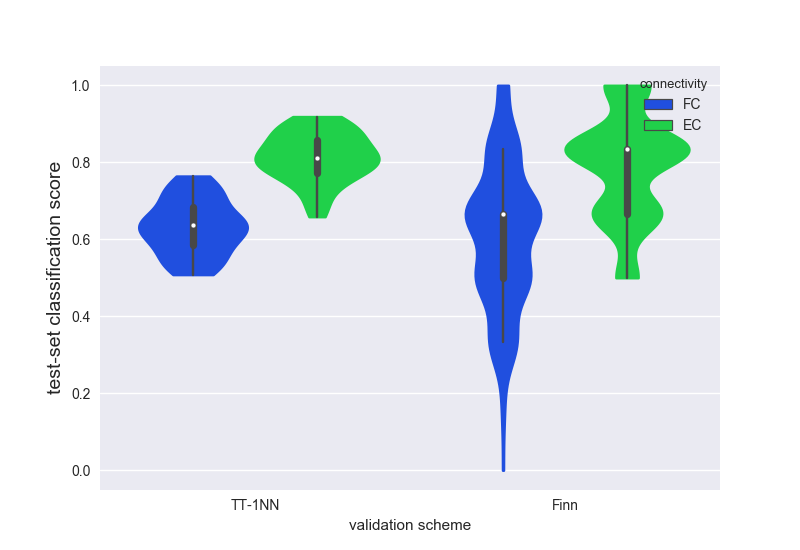
\includegraphics[width=0.89\columnwidth]{variability_finn_1nn_violins_hues}
  \caption[Variability of generalization score]{Distribution of test-set generalization score for large and small test set size.
	  \label{fig:variability_score}}
\end{center}
\end{figure}

\subsection{Comparison of classification pipelines for subjects' identity classification}
\subsubsection{z-score}
\subsubsection{PCA}
\subsubsection{Different classifiers}

\begin{figure}[!htb]
\begin{center}
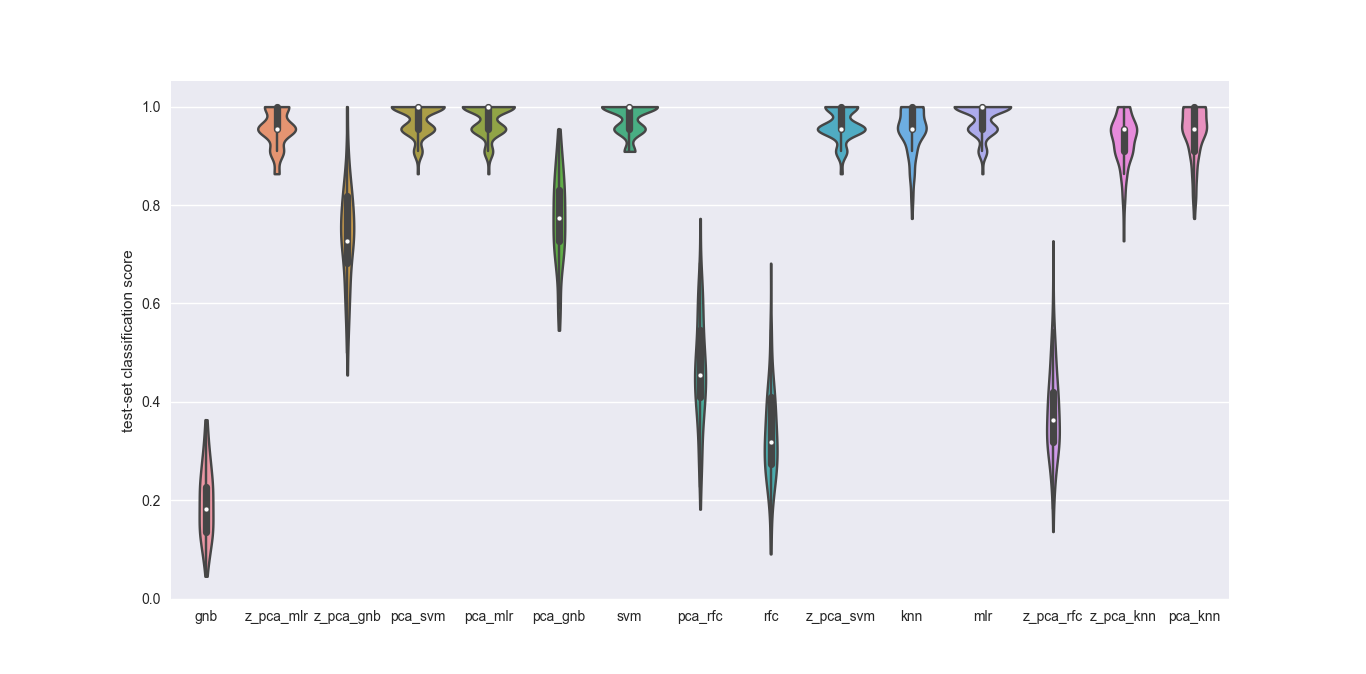
\includegraphics[width=0.89\columnwidth]{comparison_clf_subj_moviedata}
  \caption[Comparison of classifiers]{Comparison of classifiers.
	  \label{fig:clf_comp}}
\end{center}
\end{figure}
\subsection{Feature selection}
\subsubsection{Information filters}
\subsubsection{Randomized Lasso}
\subsubsection{Recursive feature elimination}

\subsection{Probabilistic class assignment and confidence as graded diagnostics measures}
\begin{figure}[!htb]
\begin{center}
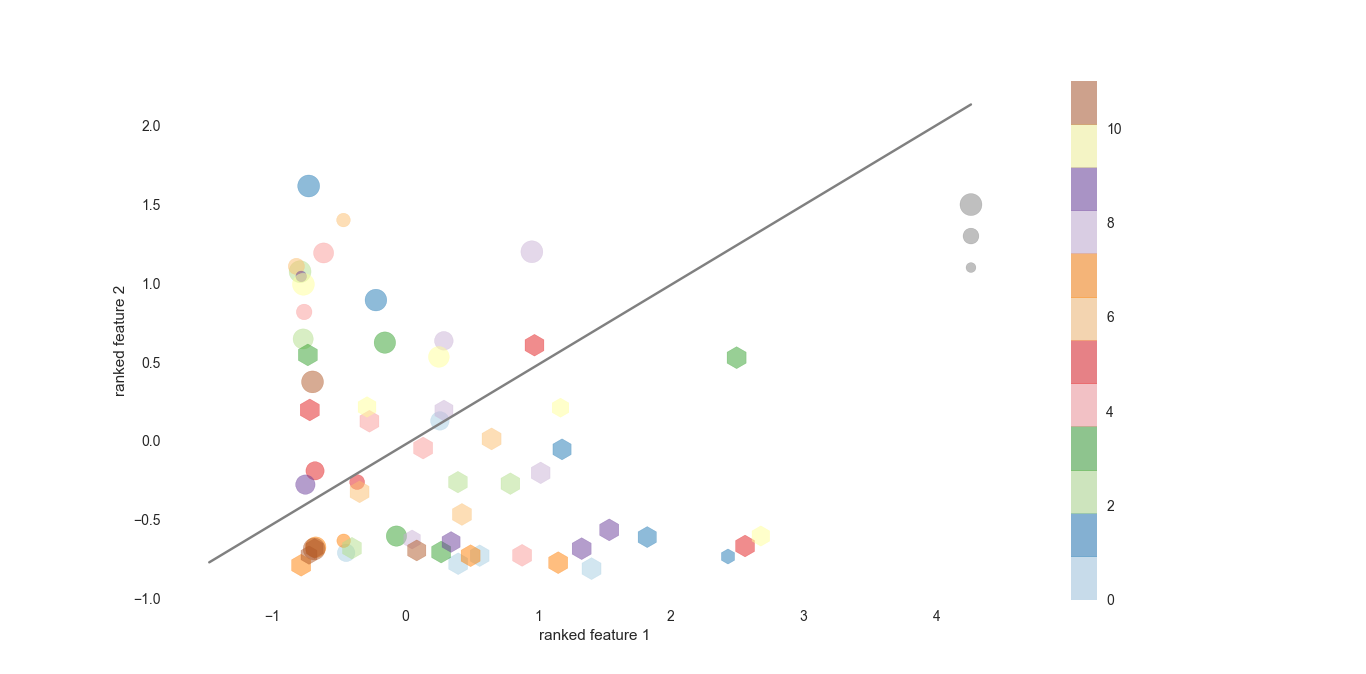
\includegraphics[width=0.89\columnwidth]{proba_samples_two_features}
  \caption[Probability of class assignment]{Probability of class assignment.
	  \label{fig:probabilistic}}
\end{center}
\end{figure}

\section{Discussion}
\label{discussion}

\textcolor{red}{resume of the results}

\textcolor{red}{explain why they are relevant}

\textcolor{red}{discuss generality, dependence on parameters, etc.}

\textcolor{red}{discuss other possible approaches (other models, methods, etc.)}

\textcolor{red}{possible applications to other fields, themes, etc.}

\textcolor{red}{other collateral themes}

\textcolor{red}{discuss future directions}

\section*{Acknowledgments}

We thank\dots 




\clearpage

%%% References
\bibliographystyle{abbrvnat}%{apalike}%{plainnat}
\bibliography{../BIB/DecisionConfidence.bib,../BIB/refs_plosReview.bib,../BIB/projThesis.bib,../BIB/refs.bib} %
%\bibliography{../BIB/DecisionConfidence.bib,../BIB/refs_plosReview.bib,../BIB/projThesis.bib,../BIB/refs.bib} %



\end{document}
